\section{problem 6}
\subsection{1.}
Using python, the signal is read in, thereafter mean and power is calculated
\begin{lstlisting}
    import numpy as np
    import matplotlib.pyplot as plt
    from scipy.signal import correlate, correlation_lags

    x = np.loadtxt("dataset.dat")
    N = len(x)

    print("mean:", np.mean(x))
    print("power:", np.mean(x**2))

    x0 = x - np.mean(x)  #remove the mean from the signal
    #correlate(x,y), we correlate the first signal with itself
    rxx = correlate(x0,x0,mode="full") / N  #correlation gives a sum of products, dividing turn into average
    #same as correlate(x,y), correlate the two function inputs.
    lags = correlation_lags(N,N, mode="full")

    #page 187, "meaningfull measure of similarity for small lags -> 20%"
    max_lag = 400
    #keep only samples that are within the bounds of a given lag
    mask = (lags >= -max_lag) & (lags <= max_lag)

    #white noise signal
    P = np.mean(x0**2) #compute mean power from the datasett
    w = np.random.normal(
    loc=0,              #noise has a mean of 0
    scale=np.sqrt(P),   #std is square root of power
    size=N              #amount of samples
    )
\end{lstlisting}
\begin{figure}[!htb]
    \centering
    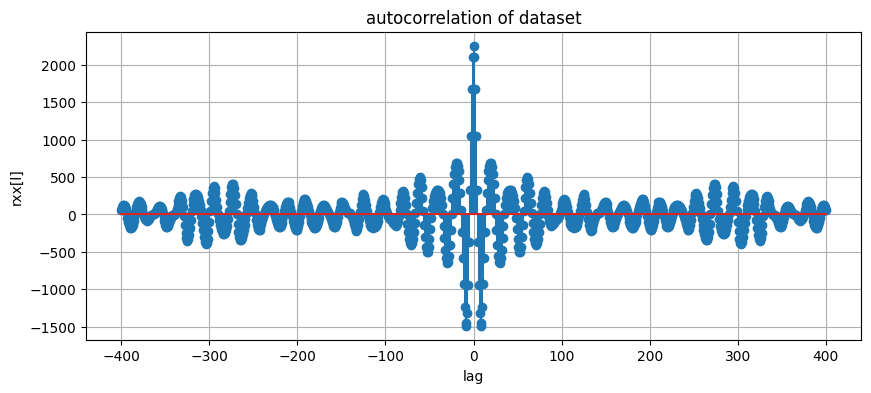
\includegraphics[width=0.7\textwidth]{p6_autocorrelation.png}
    \caption{Above is the plot of the autocorrelated data from the dataset.
    A sharp center can be seen, meaning that there is a point where 
    there is a strong correlation between itself, however there is also clear sidelobes,
    that could indicate some period elements in the dataset, meaning a slightly stronger 
    correlation elsewhere aswell.  }
\end{figure}

\begin{figure}[!htb]
    \centering
    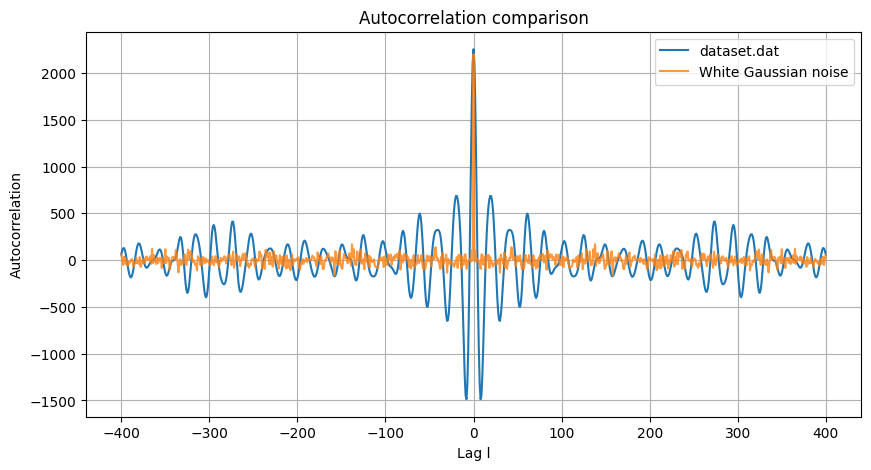
\includegraphics[width=0.7\textwidth]{p6_comparison.png}
    \caption{When comparing the autocorrelation of white noise to the dataset signal,
    it is clear that there is a singular place where the signal is a perfect match, so the autocorrelation
    of a white noise guassian signal has a clear maximum at lag 0.}
\end{figure}